\item[(d)]
\section{Direct-Form I Implementation}

\subsection*{Problem Statement}
Draw the block diagram of a direct-form I implementation of the filter and specify the coefficient values in the block diagram.

\subsection*{Theoretical Background}
A direct-form I implementation of a digital filter uses the difference equation directly to realize the filter structure. It involves using delay elements, multipliers for coefficients, and adders.

Given the transfer function in terms of \( z^{-1} \):
\[ H(z) = \frac{1 + z^{-1} + z^{-2} + z^{-3}}{1 - 1.5z^{-1} + 0.625z^{-2}} \]

The difference equation is:
\[ y[n] = x[n] + x[n-1] + x[n-2] + x[n-3] - 1.5y[n-1] + 0.625y[n-2] \]

\subsection*{Block Diagram}
The block diagram of the direct-form I implementation is shown below:

\begin{figure}[h]
    \centering
    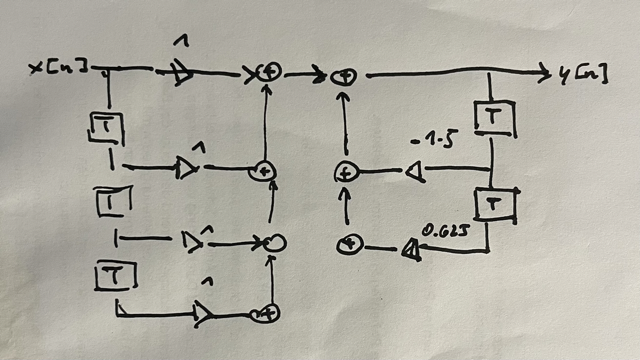
\includegraphics[width=0.8\textwidth]{fig/ex3_d_block_diagram.png}
    \caption{Block Diagram of Direct-Form I Implementation}
    \label{fig:ex3_d_block_diagram}
\end{figure}

\subsection*{Conclusion}
The block diagram of the direct-form I implementation illustrates the structure of the digital filter using delay elements, multipliers, and adders. The coefficient values are specified according to the difference equation.
